\documentclass[12pt,a4paper]{article}
\usepackage[utf8]{inputenc}
\usepackage[portuguese]{babel}
\usepackage{geometry}
\usepackage{titlesec}
\usepackage{enumitem}
\usepackage{xcolor}
\usepackage{listings}
\usepackage{graphicx}
\usepackage{hyperref}
\usepackage{booktabs}
\usepackage{longtable}
\usepackage{array}

\geometry{margin=2.5cm}
\titleformat{\section}{\Large\bfseries}{\thesection}{1em}{}
\titleformat{\subsection}{\large\bfseries}{\thesubsection}{1em}{}
\titleformat{\subsubsection}{\normalsize\bfseries}{\thesubsubsection}{1em}{}

\lstset{
    basicstyle=\ttfamily\footnotesize,
    breaklines=true,
    frame=single,
    backgroundcolor=\color{gray!10}
}

\title{\textbf{Projeto Físico de Banco de Dados}\\
\large Sistema de Gestão de Feiras}
\author{Higor Roger de Freitas Santos \quad 221006440\\
Victor Eneias Oliveira \quad 221038364\\
\\
Engenharia de Software CIC0105 Turma 01 2025.1}
\date{\today}

\begin{document}

\maketitle

\tableofcontents
\newpage

\section{Visão Geral}

Este documento apresenta o banco de dados do Sistema de Gestão de Feiras. O banco usa SQLite e possui 5 tabelas principais que armazenam todas as informações necessárias para o funcionamento do sistema.

\subsection{Características do Banco}

\begin{itemize}
    \item \textbf{Banco}: SQLite (arquivo único, fácil de usar)
    \item \textbf{Tabelas}: 5 tabelas principais conectadas entre si
    \item \textbf{Segurança}: Cada registro tem um dono (id\_criador)
    \item \textbf{Organização}: Dados bem organizados sem repetição
\end{itemize}

\subsection{Como as Tabelas se Conectam}

\begin{itemize}
    \item Todas as tabelas têm um campo \textbf{id} que é único
    \item O campo \textbf{id\_criador} mostra quem criou cada registro
    \item As tabelas se conectam através de campos como \textbf{feira\_id}, \textbf{expositor\_id}
\end{itemize}

\section{Diagrama do Banco de Dados}

O diagrama abaixo mostra como as 5 tabelas se relacionam:

\begin{figure}[htbp]
    \centering
    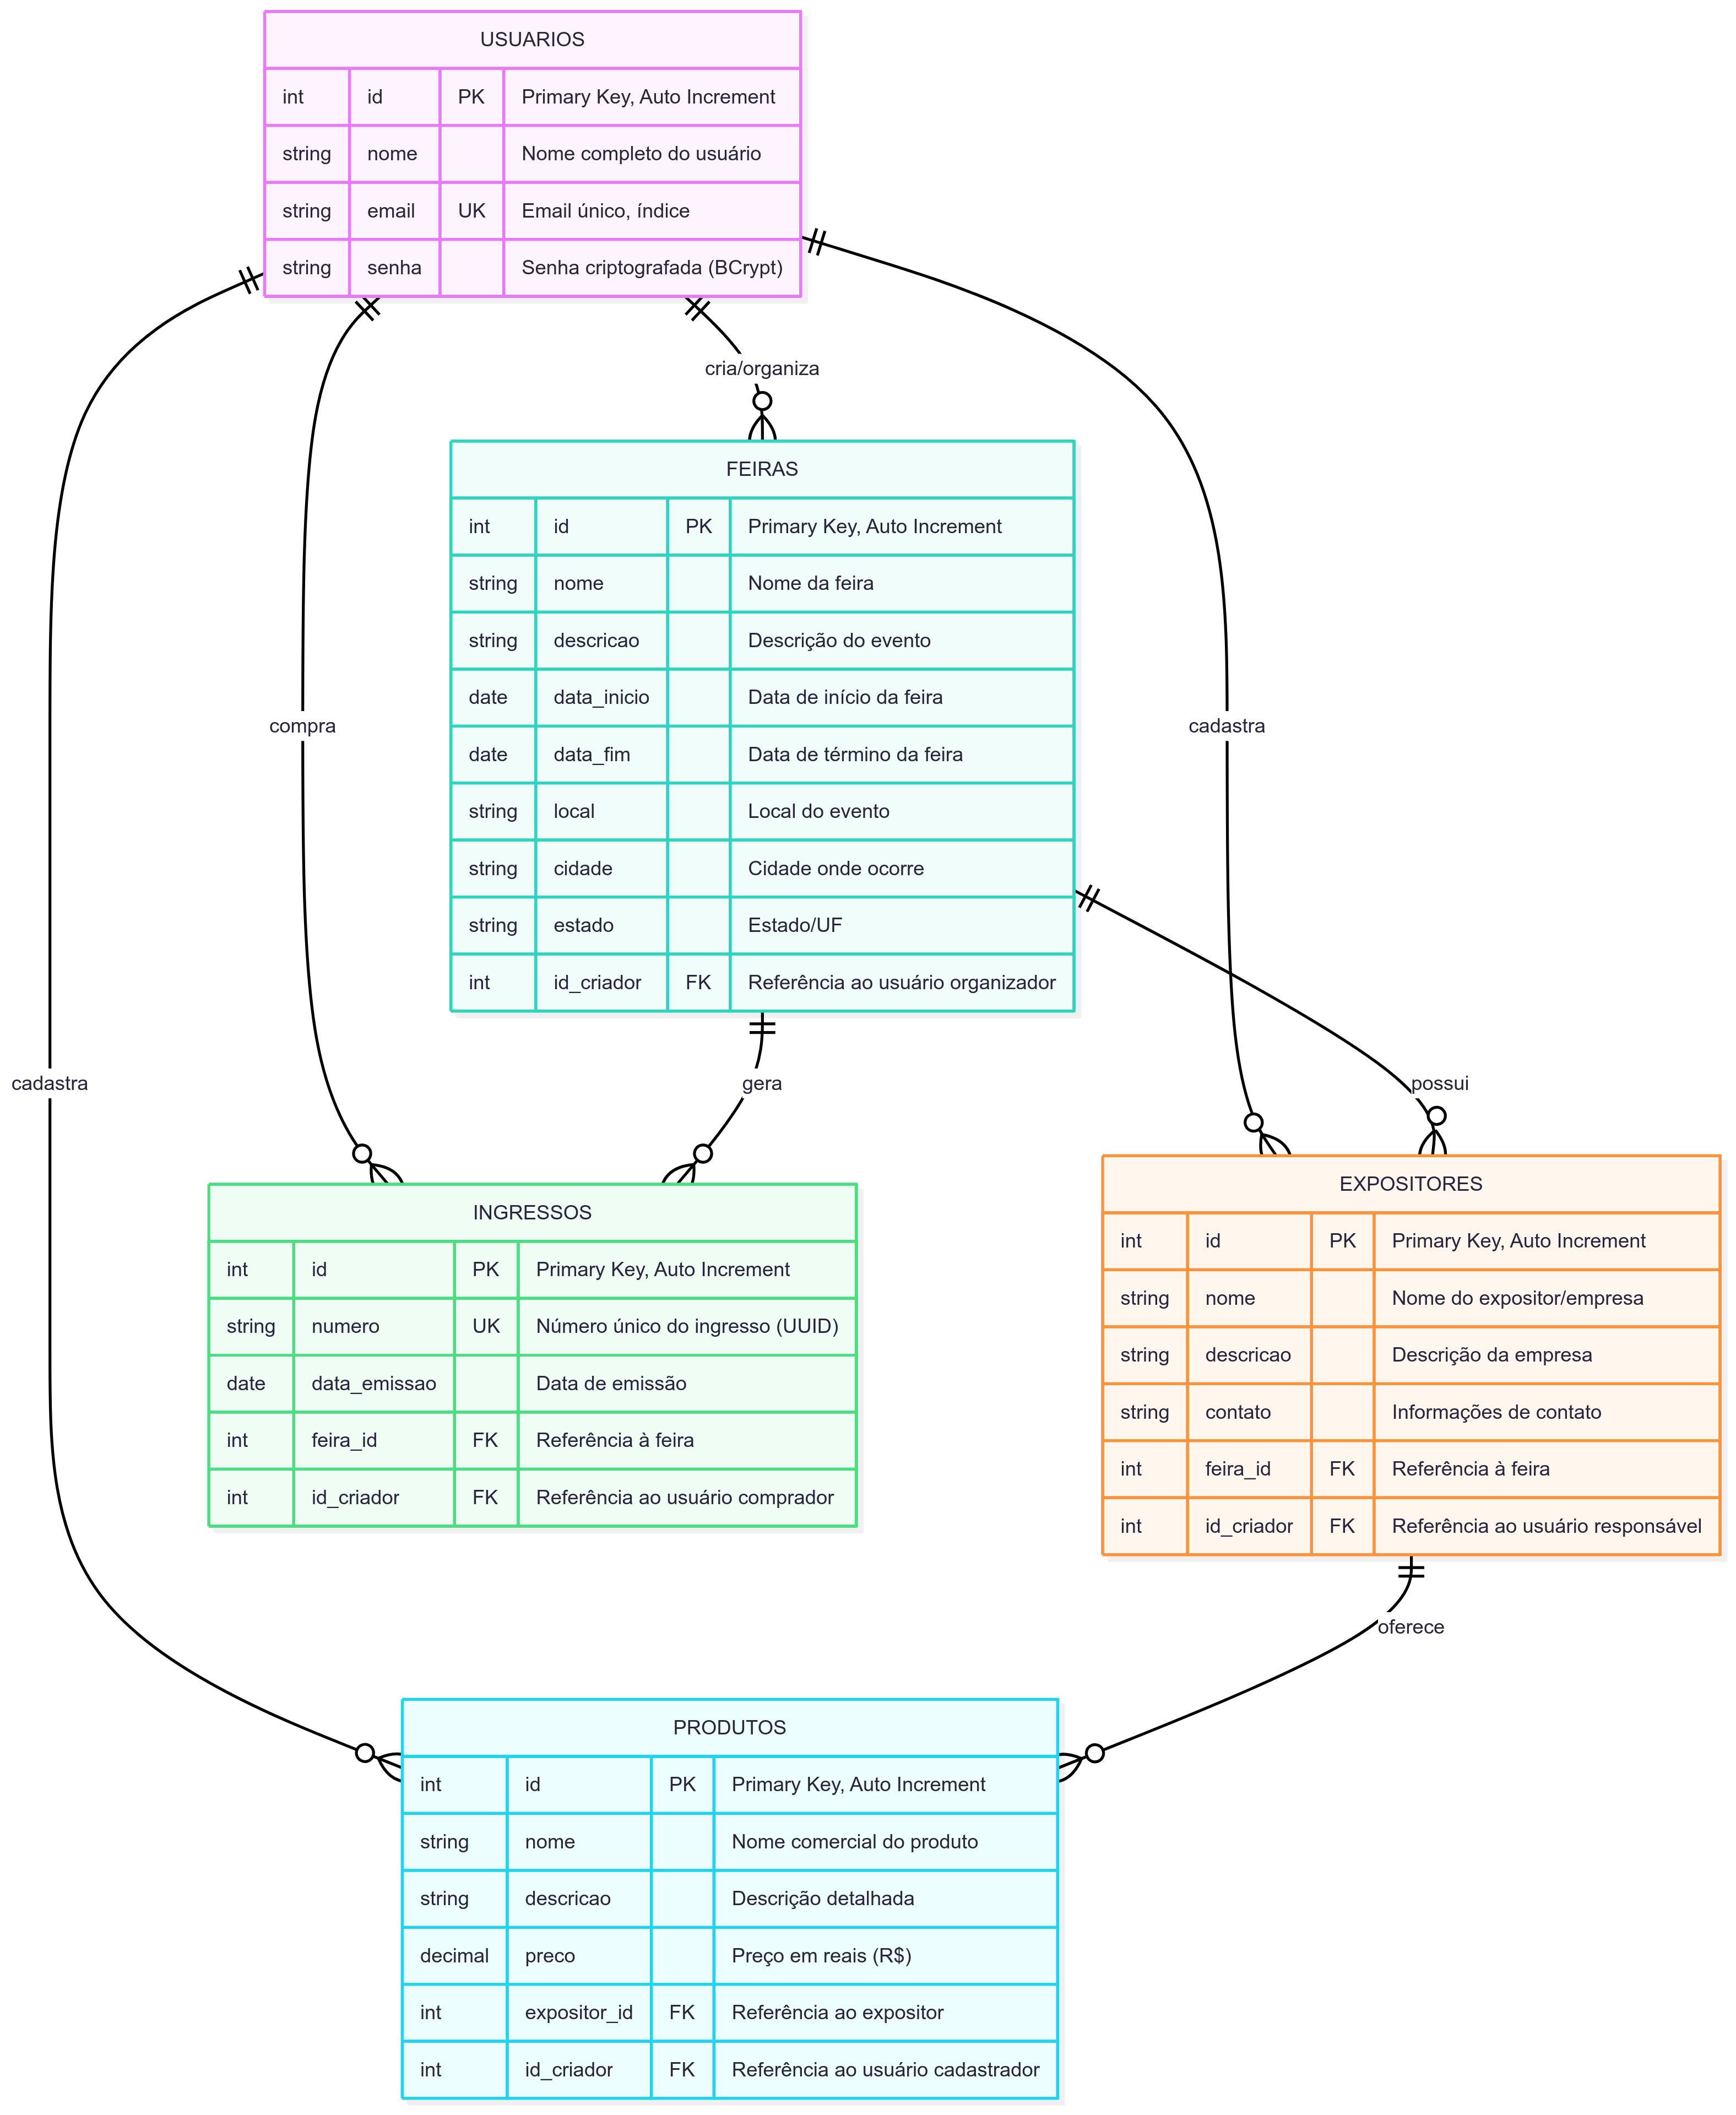
\includegraphics[width=0.9\textwidth]{diagrams/banco_dados_er.png}
    \caption{Estrutura do Banco de Dados}
    \label{fig:diagrama_er}
\end{figure}

\section{Descrição das Tabelas}

\subsection{Tabela: usuarios}

\textbf{Para que serve}: Guarda os dados de login dos usuários do sistema.

\begin{longtable}{|p{3cm}|p{2cm}|p{2cm}|p{1.5cm}|p{5cm}|}
\hline
\textbf{Campo} & \textbf{Tipo} & \textbf{Tamanho} & \textbf{Obrigat.} & \textbf{Descrição} \\
\hline
\endhead
id & INTEGER & -- & SIM & Número único do usuário \\
\hline
nome & VARCHAR & 255 & SIM & Nome completo \\
\hline
email & VARCHAR & 255 & SIM & Email para login (único) \\
\hline
senha & VARCHAR & 255 & SIM & Senha criptografada \\
\hline
\end{longtable}

\textbf{Regras importantes}:
\begin{itemize}
    \item Cada email só pode ser usado uma vez
    \item A senha é guardada criptografada por segurança
\end{itemize}

\subsection{Tabela: feiras}

\textbf{Para que serve}: Guarda informações sobre as feiras (eventos).

\begin{longtable}{|p{3cm}|p{2cm}|p{2cm}|p{1.5cm}|p{5cm}|}
\hline
\textbf{Campo} & \textbf{Tipo} & \textbf{Tamanho} & \textbf{Obrigat.} & \textbf{Descrição} \\
\hline
\endhead
id & INTEGER & -- & SIM & Número único da feira \\
\hline
nome & VARCHAR & 255 & SIM & Nome da feira \\
\hline
descricao & TEXT & -- & NÃO & Descrição do evento \\
\hline
data\_inicio & DATE & -- & SIM & Quando começa \\
\hline
data\_fim & DATE & -- & SIM & Quando termina \\
\hline
local & VARCHAR & 255 & SIM & Onde acontece \\
\hline
cidade & VARCHAR & 100 & SIM & Cidade \\
\hline
estado & VARCHAR & 2 & SIM & Estado (SP, RJ, etc.) \\
\hline
id\_criador & INTEGER & -- & SIM & Quem criou a feira \\
\hline
\end{longtable}

\textbf{Regras importantes}:
\begin{itemize}
    \item A data de fim deve ser depois da data de início
    \item Só quem criou a feira pode editá-la
\end{itemize}

\subsection{Tabela: expositores}

\textbf{Para que serve}: Guarda dados das empresas que participam das feiras.

\begin{longtable}{|p{3cm}|p{2cm}|p{2cm}|p{1.5cm}|p{5cm}|}
\hline
\textbf{Campo} & \textbf{Tipo} & \textbf{Tamanho} & \textbf{Obrigat.} & \textbf{Descrição} \\
\hline
\endhead
id & INTEGER & -- & SIM & Número único do expositor \\
\hline
nome & VARCHAR & 255 & SIM & Nome da empresa \\
\hline
descricao & TEXT & -- & NÃO & O que a empresa faz \\
\hline
contato & VARCHAR & 255 & SIM & Telefone, email, etc. \\
\hline
feira\_id & INTEGER & -- & SIM & Em qual feira participa \\
\hline
id\_criador & INTEGER & -- & SIM & Quem cadastrou \\
\hline
\end{longtable}

\textbf{Regras importantes}:
\begin{itemize}
    \item Cada expositor participa de uma feira específica
    \item Só quem cadastrou pode editar os dados
\end{itemize}

\subsection{Tabela: produtos}

\textbf{Para que serve}: Lista os produtos que cada expositor oferece.

\begin{longtable}{|p{3cm}|p{2cm}|p{2cm}|p{1.5cm}|p{5cm}|}
\hline
\textbf{Campo} & \textbf{Tipo} & \textbf{Tamanho} & \textbf{Obrigat.} & \textbf{Descrição} \\
\hline
\endhead
id & INTEGER & -- & SIM & Número único do produto \\
\hline
nome & VARCHAR & 255 & SIM & Nome do produto \\
\hline
descricao & TEXT & -- & NÃO & Detalhes do produto \\
\hline
preco & DECIMAL & (10,2) & SIM & Preço em reais \\
\hline
expositor\_id & INTEGER & -- & SIM & De qual expositor \\
\hline
id\_criador & INTEGER & -- & SIM & Quem cadastrou \\
\hline
\end{longtable}

\textbf{Regras importantes}:
\begin{itemize}
    \item O preço deve ser maior que zero
    \item Cada produto pertence a um expositor
\end{itemize}

\subsection{Tabela: ingressos}

\textbf{Para que serve}: Controla os ingressos vendidos para as feiras.

\begin{longtable}{|p{3cm}|p{2cm}|p{2cm}|p{1.5cm}|p{5cm}|}
\hline
\textbf{Campo} & \textbf{Tipo} & \textbf{Tamanho} & \textbf{Obrigat.} & \textbf{Descrição} \\
\hline
\endhead
id & INTEGER & -- & SIM & Número único do ingresso \\
\hline
numero & VARCHAR & 36 & SIM & Código do ingresso \\
\hline
data\_emissao & DATE & -- & SIM & Quando foi comprado \\
\hline
feira\_id & INTEGER & -- & SIM & Para qual feira \\
\hline
id\_criador & INTEGER & -- & SIM & Quem comprou \\
\hline
\end{longtable}

\textbf{Regras importantes}:
\begin{itemize}
    \item Cada ingresso tem um código único
    \item Cada ingresso é válido para uma feira específica
\end{itemize}

\section{Como as Tabelas se Relacionam}

\begin{enumerate}
    \item \textbf{Usuario cria Feiras}: Um usuário pode organizar várias feiras
    \item \textbf{Usuario cadastra Expositores}: Um usuário pode cadastrar vários expositores
    \item \textbf{Feira tem Expositores}: Uma feira pode ter vários expositores
    \item \textbf{Expositor oferece Produtos}: Um expositor pode ter vários produtos
    \item \textbf{Usuario compra Ingressos}: Um usuário pode comprar vários ingressos
    \item \textbf{Feira gera Ingressos}: Uma feira pode ter vários ingressos vendidos
\end{enumerate}

\newpage

\section{Scripts para Criar o Banco}

\subsection{Criação das Tabelas}

\begin{lstlisting}[language=SQL, caption=Como criar as tabelas]
-- Tabela de usuarios
CREATE TABLE usuarios (
    id INTEGER PRIMARY KEY AUTOINCREMENT,
    nome VARCHAR(255) NOT NULL,
    email VARCHAR(255) NOT NULL UNIQUE,
    senha VARCHAR(255) NOT NULL
);

-- Tabela de feiras
CREATE TABLE feiras (
    id INTEGER PRIMARY KEY AUTOINCREMENT,
    nome VARCHAR(255) NOT NULL,
    descricao TEXT,
    data_inicio DATE NOT NULL,
    data_fim DATE NOT NULL,
    local VARCHAR(255) NOT NULL,
    cidade VARCHAR(100) NOT NULL,
    estado VARCHAR(2) NOT NULL,
    id_criador INTEGER NOT NULL,
    FOREIGN KEY (id_criador) REFERENCES usuarios(id)
);

-- Tabela de expositores
CREATE TABLE expositores (
    id INTEGER PRIMARY KEY AUTOINCREMENT,
    nome VARCHAR(255) NOT NULL,
    descricao TEXT,
    contato VARCHAR(255) NOT NULL,
    feira_id INTEGER NOT NULL,
    id_criador INTEGER NOT NULL,
    FOREIGN KEY (feira_id) REFERENCES feiras(id),
    FOREIGN KEY (id_criador) REFERENCES usuarios(id)
);

-- Tabela de produtos
CREATE TABLE produtos (
    id INTEGER PRIMARY KEY AUTOINCREMENT,
    nome VARCHAR(255) NOT NULL,
    descricao TEXT,
    preco DECIMAL(10,2) NOT NULL CHECK (preco > 0),
    expositor_id INTEGER NOT NULL,
    id_criador INTEGER NOT NULL,
    FOREIGN KEY (expositor_id) REFERENCES expositores(id),
    FOREIGN KEY (id_criador) REFERENCES usuarios(id)
);

-- Tabela de ingressos
CREATE TABLE ingressos (
    id INTEGER PRIMARY KEY AUTOINCREMENT,
    numero VARCHAR(36) NOT NULL UNIQUE,
    data_emissao DATE NOT NULL,
    feira_id INTEGER NOT NULL,
    id_criador INTEGER NOT NULL,
    FOREIGN KEY (feira_id) REFERENCES feiras(id),
    FOREIGN KEY (id_criador) REFERENCES usuarios(id)
);
\end{lstlisting}

\subsection{Indices para Busca Rapida}

\begin{lstlisting}[language=SQL, caption=Indices para melhorar a velocidade]
-- Indices para buscar mais rapido
CREATE INDEX idx_feiras_criador ON feiras(id_criador);
CREATE INDEX idx_expositores_feira ON expositores(feira_id);
CREATE INDEX idx_expositores_criador ON expositores(id_criador);
CREATE INDEX idx_produtos_expositor ON produtos(expositor_id);
CREATE INDEX idx_produtos_criador ON produtos(id_criador);
CREATE INDEX idx_ingressos_feira ON ingressos(feira_id);
CREATE INDEX idx_ingressos_criador ON ingressos(id_criador);
\end{lstlisting}

\end{document}
